\documentclass[conference,a4paper]{IEEEtran}
\usepackage[T1]{fontenc}
\usepackage[utf8]{inputenc}
\usepackage{url}
\usepackage{amsmath}
\usepackage{booktabs}
\usepackage{array}
\usepackage{balance}
\usepackage{tikz}
\usetikzlibrary{arrows.meta,positioning}
\usepackage[hidelinks]{hyperref}
\hypersetup{pdftitle={Single-Cycle RV32I Processor},pdfauthor={Viraj, Kaustubh, Pratyush, Bhargav and Rudraksh}}
\Urlmuskip=0mu plus 1mu
\renewcommand{\ttdefault}{cmtt}

\title{Single-Cycle RV32I Processor:\\Design, Verification and Generic Synthesis}

\author{
\IEEEauthorblockN{Viraj, Kaustubh, Pratyush, Bhargav and Rudraksh}
\IEEEauthorblockA{Student Project Team\\
Affiliation not supplied for this review copy}
}

\begin{document}
\maketitle\thispagestyle{plain}\pagestyle{plain}
\begin{center}\footnotesize\textit{Review copy: official full names, affiliation and academic Phase I cutoff require confirmation. Results below describe the completed development milestones, not an assumed Phase I submission date.}\end{center}

\begin{abstract}
This paper presents a modular single-cycle processor executing ten selected
RV32I instructions in Verilog-2001. The design integrates a 32-bit program
counter, separate instruction and data memories, an exact decoder, a 32-register
file, immediate generation, an arithmetic and logic unit, branch selection and
memory writeback. Diagnostic fault gating suppresses side effects on invalid
fetches, instructions and data addresses. Sixteen self-checking testbenches
report 276,741 passing HDL checks; a 38-instruction integration program is compared
cycle by cycle with an independent architectural reference. Generic Yosys
synthesis reports 22,695 leaf generic cells and no inferred latches. A separate
port-observable simulation of the generated netlist passes 163 checks and
confirms a correction to ROM synthesis initialization. The implementation is an
educational instruction subset, not a full RV32I-compliant processor. Results
are bounded to tested behavior and generic synthesis; device utilization, maximum
clock frequency, power and FPGA deployment have not been measured.
\end{abstract}
\begin{IEEEkeywords}
RISC-V, RV32I subset, single-cycle processor, Verilog, simulation, logic synthesis.
\end{IEEEkeywords}

\section{Introduction and Objectives}
The objective is to expose instruction fetch, decode, operand selection,
execution, memory access and writeback in a compact single-cycle processor.
All of these functions complete within one cycle; they are not pipeline stages.
The supported instructions are ADD, SUB, AND, OR, XOR, ADDI, LW, SW, BEQ and BNE.
Other RV32I instructions, privileged traps, interrupts and caches are outside
scope. The diagnostic fault mechanism is a teaching feature, not an implementation
of machine-mode exceptions.

Separate instruction ROM and data RAM permit concurrent instruction fetch and
data access. Invalid fetches, unsupported encodings, invalid RAM addresses and
taken misaligned branches suppress side effects. Causes 01, 10 and 11 distinguish
fetch, instruction and data/branch faults. A synchronous reset clears the fault.
The design aims at inspectable behavior and reproducibility rather than measured
performance superiority over other processors.

\section{Literature Review}
The RV32I chapter, Version 2.1, of the RISC-V Unprivileged ISA specification
(release v20260120)~\cite{ref1} defines the architectural contract independently
of the implementation: register x0, instruction fields, immediate formats and
operation semantics. Those definitions guide the decoder and reference model.
Icarus documentation~\cite{ref2} supports the event-driven verification workflow,
while Yosys documentation~\cite{ref3} distinguishes generic synthesis from
hardware-specific mapping. Simulation validates selected behavior; synthesis
provides complementary structural and generic resource evidence.

The supplied MIPS designs~\cite{ref4} informed modular organization only.
Their encodings, control matrices, authorship and results are not this project's
RISC-V implementation or evidence. This review uses primary specifications and
tool documentation; no unperformed research benchmark comparison is claimed.

\section{Proposed Solution and Implementation}
The single-cycle RV32I processor is organized into distinct, modular functional blocks interconnected by dedicated 32-bit buses.

A 32-bit Program Counter (\texttt{pc.v}) resets synchronously to \texttt{32'h00000000} and advances to \texttt{next\_pc} on each clock edge when unhalted. A 256-word instruction read-only memory (\texttt{instruction\_memory.v}) is combinationally addressed by \texttt{pc[9:2]}, returning the 32-bit instruction word within the cycle while enforcing 4-byte alignment (\texttt{pc[1:0] == 2'b00}) and range bounds (\texttt{0x000}--\texttt{0x3FC}).

The control unit and decoder (\texttt{control\_unit.v}) decodes \texttt{opcode}, \texttt{funct3}, and \texttt{funct7}, generating write enables, multiplexer select lines, and ALU operation codes. Unrecognized instruction words deassert write enables and flag an illegal instruction fault. The register file (\texttt{register\_file.v}) contains 32 registers with two asynchronous read ports and one synchronous write port; register \texttt{x0} discards writes and always reads zero. The immediate generator (\texttt{immediate\_generator.v}) produces sign-extended 32-bit immediates for I-format, S-format, and B-format (with bit 0 implicitly zero).

The arithmetic logic unit (\texttt{alu.v}) performs addition, subtraction, AND, OR, and XOR, and computes effective memory addresses for \texttt{LW} and \texttt{SW}. A dedicated branch unit (\texttt{branch\_unit.v}) compares register operands for \texttt{BEQ} and \texttt{BNE} and computes the branch target as \texttt{pc + imm\_b}. Data memory (\texttt{data\_memory.v}) provides 256 words with asynchronous reads for single-cycle \texttt{LW} writeback and synchronous writes for \texttt{SW}. The writeback multiplexer (\texttt{writeback\_mux.v}) selects between the ALU output and memory read data.

Top-level parameter \texttt{ARITHMETIC\_ONLY} is retained for backwards compatibility with Phase-3 regression tests. Programs terminate cleanly using a legal \texttt{BEQ} self-loop (\texttt{BEQ x0, x0, 0}).

\begin{figure}[t]
\centering
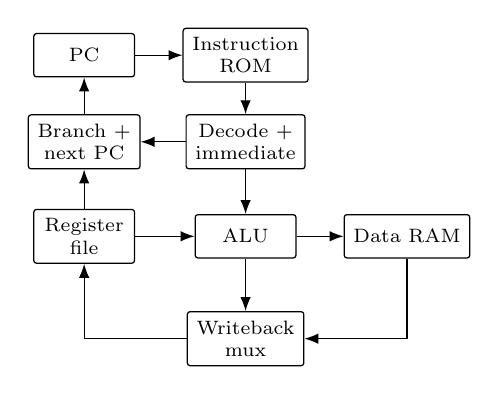
\begin{tikzpicture}[x=1cm,y=1cm,>=Latex,
 box/.style={draw,rounded corners=1pt,align=center,font=\scriptsize,minimum height=0.55cm,minimum width=1.28cm},
 every path/.style={line width=0.45pt}]
\node[box] (pc) at (0,3.7) {PC};
\node[box] (rom) at (2.05,3.7) {Instruction\\ROM};
\node[box] (dec) at (2.05,2.6) {Decode +\\immediate};
\node[box] (reg) at (0,1.4) {Register\\file};
\node[box] (alu) at (2.05,1.4) {ALU};
\node[box] (ram) at (4.1,1.4) {Data RAM};
\node[box] (wb) at (2.05,0.1) {Writeback\\mux};
\node[box] (br) at (0,2.6) {Branch +\\next PC};
\draw[->] (pc)--(rom);
\draw[->] (rom)--(dec);
\draw[->] (dec)--(alu);
\draw[->] (dec)--(br);
\draw[->] (reg)--(alu);
\draw[->] (reg)--(br);
\draw[->] (br)--(pc);
\draw[->] (alu)--(ram);
\draw[->] (alu)--(wb);
\draw[->] (ram)|-(wb);
\draw[->] (wb)-|(reg);
\end{tikzpicture}
\caption{Implemented high-level datapath. Decoder control fanout, register
indices, the rs2 store-data connection and reset/fault qualification are omitted
for clarity. ROM and RAM each hold 256 32-bit words.}
\label{fig:architecture}
\end{figure}

\section{Verification Methodology}
The verification framework combines multi-tiered testbenches executed via \path{tools/run_tests.py}:
\begin{enumerate}
\item \textbf{Instruction Encoding Checks:} Validates machine-code word encodings against bitfield disassembly rules for all supported instructions.
\item \textbf{Independent Architectural Reference:} A Python reference emulator independently executes test programs, decodes instructions, updates state, and outputs golden cycle-by-cycle execution traces.
\item \textbf{Integration Test Suite (\texttt{tb\_full\_isa.sv}):} Executes a 38-instruction program covering all ten supported operations, memory load/store sequences, and four branch outcomes (BEQ taken/not taken and BNE taken/not taken).
\item \textbf{Directed Component Testbenches:} Sixteen self-checking testbenches validate edge cases, including register file write priority, x0 write protection and load-address validation, two's-complement arithmetic overflow, branch outcome truth tables, data memory alignment, synchronous reset during a pending store (\texttt{tb\_cpu\_reset\_memory.sv}), and fault injection.
\item \textbf{Runner Integrity Checks:} Test execution strictly validates output, rejecting runs with simulator errors, missing \texttt{PASS} banners, or timeouts.
\end{enumerate}

Key technical distinctions must be emphasized:
\begin{itemize}
\item \textbf{HDL Assertions vs. Executed Instructions:} The 276,741 reported assertion checks include 262,144 combinational checks from exhaustive sweeps of the instruction decoder, evaluating control lines across bitfield permutations. These represent combinational assertion evaluations, not 262,144 executed CPU instructions. The number of fully executed CPU instructions is bounded by the specific integration programs (e.g., 38 instructions in \texttt{tb\_full\_isa.sv}).
\item \textbf{RTL Simulation vs. Netlist Simulation:} RTL simulation operates on behavioral Verilog with internal register visibility; netlist simulation operates on the gate-level netlist generated by Yosys synthesis and verifies the CPU's public debug ports, including PC/instruction, register writeback, RAM enables/data, branch decision and next-PC signals, over the 38-instruction trace.
\item \textbf{Bounded Testing vs. Formal Proof:} Bounded simulation establishes agreement with expected behavior for the tested stimuli and edge cases; it does not constitute a mathematical formal equivalence proof across all possible 32-bit execution sequences.
\end{itemize}

\section{Results and Discussion}
The recorded evidence gives the results in Table~\ref{tab:results}.
RTL regression results are pinned by input hashes in
\path{reports/verification/phase-5-manifest.json}. Synthesis and netlist evidence
are under \path{reports/synthesis/}; these were working-tree runs on the accepted
Phase-4 base, subsequently packaged in the Phase-5 implementation commit.

\begin{table}[t]
\caption{Recorded functional and generic synthesis results}
\label{tab:results}
\centering\small
\begin{tabular}{p{0.68\columnwidth}r}
\toprule
Measure & Result\\\midrule
RTL HDL checks / test suites & 276,741 / 16\\
Known encoding vectors & 10\\
Reference instructions / supported operations & 38 / 10\\
Branch outcome classes & 4\\
Port-observable netlist checks & 163\\
Hierarchical cells (includes 9 instances) & 22,704\\
Leaf generic cells & 22,695\\
Generic flip-flop cells & 9,251\\
Generic multiplexer cells & 9,555\\
Inferred latches & 0\\\bottomrule
\end{tabular}
\end{table}

The flip-flop count consists of 8,192 data-RAM bits, 1,024 register-file bits,
and 35 PC/fault-state bits. The two decoder sweeps account for 262,144 checks;
other checks exercise components, integration, faults and reset. The netlist
smoke test is reported separately from the RTL total.

\subsection{Distinction Between Generic Cells and FPGA Resources}
Generic cells are abstract, technology-independent Boolean primitives. They do not correspond directly to FPGA Look-Up Tables (LUTs), Configurable Logic Blocks (CLBs), or dedicated hardware Block RAMs (BRAMs). The 8,192 flip-flops in data memory arise because single-cycle load writeback requires asynchronous read access; standard FPGA BRAMs require a synchronous read edge. This generic synthesis run does not perform place-and-route or device-specific timing closure.

\subsection{ROM Synthesis Defect and Regression}
During Phase-5 synthesis, an initialization flaw was uncovered: in behavioral simulation, ROM words were initialized to NOPs via a procedural loop before loading via \texttt{\$readmemh}. In Yosys structural synthesis, this procedural loop masked the \texttt{\$readmemh} contents, causing the synthesized ROM netlist to contain all NOPs. Netlist simulation detected this immediately on cycle 1, observing \texttt{00000013} instead of \texttt{04000093}. The lead corrected \texttt{instruction\_memory.v} by separating synthesis and simulation initialization paths. Following correction, the synthesized netlist passed all 163 port-observable checks over the 38-instruction trace. This RTL correction was authored by Viraj as part of the lead implementation; Rudraksh audited and verified the evidence.

\section{Performance Observations}
In this single-cycle processor, every valid non-faulting instruction executes and commits state updates on a single rising clock edge:
\begin{equation}
\text{CPI} = 1.0
\end{equation}
Fault holds and synchronous reset freeze execution rather than retiring instructions, and thus do not represent a multi-cycle CPI penalty.

A CPI of 1.0 does not imply high clock frequency. The achievable clock frequency ($F_{\max}$) is constrained by the long combinational propagation path. Testbench clock periods (e.g., 10~ns / 100~MHz) are arbitrary simulation timescale parameters and do not represent measured hardware frequency.

A plausible critical-path candidate is the Load Word (\texttt{LW}) path; no target-specific timing analysis has established the longest path:
\begin{equation}
\begin{aligned}
T_{\mathrm{clk}} \geq {}&T_{\mathrm{pc}}+T_{\mathrm{ROM}}+T_{\mathrm{decode}}+T_{\mathrm{reg}}\\
 &+T_{\mathrm{ALU}}+T_{\mathrm{RAM}}+T_{\mathrm{mux}}+T_{\mathrm{setup}} .
\end{aligned}
\end{equation}
Because instruction fetch, decode, register read, ALU effective address addition, RAM read, writeback multiplexing, and register setup all occur within one clock period, this long combinational delay inherently limits hardware clock speed. Determining an actual $F_{\max}$, setup/hold slack, or dynamic power requires physical synthesis and target-specific Static Timing Analysis (STA).

\balance
\section{Individual Contributions}
Table~\ref{tab:members} records the responsibilities supported by the cumulative
Git history. The lead implemented RTL, benches and build tools. Other members'
documentation contributions do not imply authorship of those implementation files.
Initial drafts used assistant support; member commits record subsequent report,
reference, checklist and explanation changes. Personal execution or interview
readiness is not inferred from commit counts.

\begin{table}[t]
\caption{Team responsibilities and contribution areas}
\label{tab:members}
\centering\small
\begin{tabular}{p{0.20\columnwidth}p{0.70\columnwidth}}
\toprule Member & Contribution area\\\midrule
Viraj & Architecture, RTL, tests, tools, synthesis and ROM fix\\
Kaustubh & Instruction reference, encodings and worked examples\\
Pratyush & Datapath, control signals and validation explanations\\
Bhargav & Test plan, results, waveform documentation and handoff\\
Rudraksh & Reports, references, checklists, demo script and interview notes\\\bottomrule
\end{tabular}
\end{table}

\section{Conclusion}
The processor demonstrates ten selected RV32I instructions with modular control,
checked memory access and diagnostic fault gating. The recorded RTL regression,
reference trace and netlist smoke test support the tested behavior; generic
synthesis reports structure and resources without establishing device timing.
Full ISA compliance, formal equivalence and FPGA deployment are not claimed.
Before academic submission, confirm author/affiliation details and the Phase I
cutoff, obtain team approval and check the linked video's duration and access.
This final-development report must not be backdated to an unconfirmed cutoff.

\section*{Acknowledgment}
The supplied IEEEtran manuscript guided layout and organization only. Its team
identities, figures and memory-comparison results were not reused. Assistant
support and individual contribution boundaries are disclosed above.

\begin{thebibliography}{4}
\bibitem{ref1} RISC-V International, ``RV32I Base Integer Instruction Set, Version 2.1,'' in \emph{The RISC-V Instruction Set Manual, Volume I: Unprivileged ISA}, release v20260120, Jan. 2026. \url{https://docs.riscv.org/reference/isa/v20260120/unpriv/rv32.html}
\bibitem{ref2} S. Williams and contributors, ``Icarus Verilog Documentation and User Guide,'' Release Documentation, 2026. \url{https://steveicarus.github.io/iverilog/}
\bibitem{ref3} C. Wolf and YosysHQ, ``Yosys Command Reference and Synthesis Manual,'' YosysHQ Documentation, 2026. \url{https://yosyshq.readthedocs.io/projects/yosys/en/latest/using_yosys/synthesis/synth.html}
\bibitem{ref4} Project Team, ``Source Provenance and Architectural References,'' repository \texttt{REFERENCES.md}, Nov. 2026.
\end{thebibliography}

\end{document}
